\begin{frame}[fragile]{Tutorial: Two-site state optimization}

\begin{columns}

\begin{column}{5cm}

\begin{onlyenv}<1->
\begin{lstlisting}[language=JuliaLocal, style=julia, mathescape, basicstyle=\small]
function E($\psi$)
  $\psi$H$\psi$ = inner($\psi$', H, $\psi$)
  $\psi$$\psi$ = inner($\psi$, $\psi$)
  return $\psi$H$\psi$ / $\psi$$\psi$
end
\end{lstlisting}
\end{onlyenv}

\begin{onlyenv}<3->
\begin{lstlisting}[language=JuliaLocal, style=julia, mathescape, basicstyle=\small]
function minimize(f, $\partial$f, x;
  nsteps, $\gamma$)
  for n in 1:nsteps
    x = x - $\gamma$ * $\partial$f(x)
  end
  return x
end
\end{lstlisting}
\end{onlyenv}

\end{column}

\begin{column}{5cm}

\begin{onlyenv}<1-1>
Function to minimize: \\
Expectation value of the \\
energy. \\
~\\
E($\psi$) = $\langle$$\psi$|H|$\psi$$\rangle$/$\langle$$\psi$|$\psi$$\rangle$
\end{onlyenv}

\begin{onlyenv}<2->
\vspace*{0.0cm}
\begin{center}
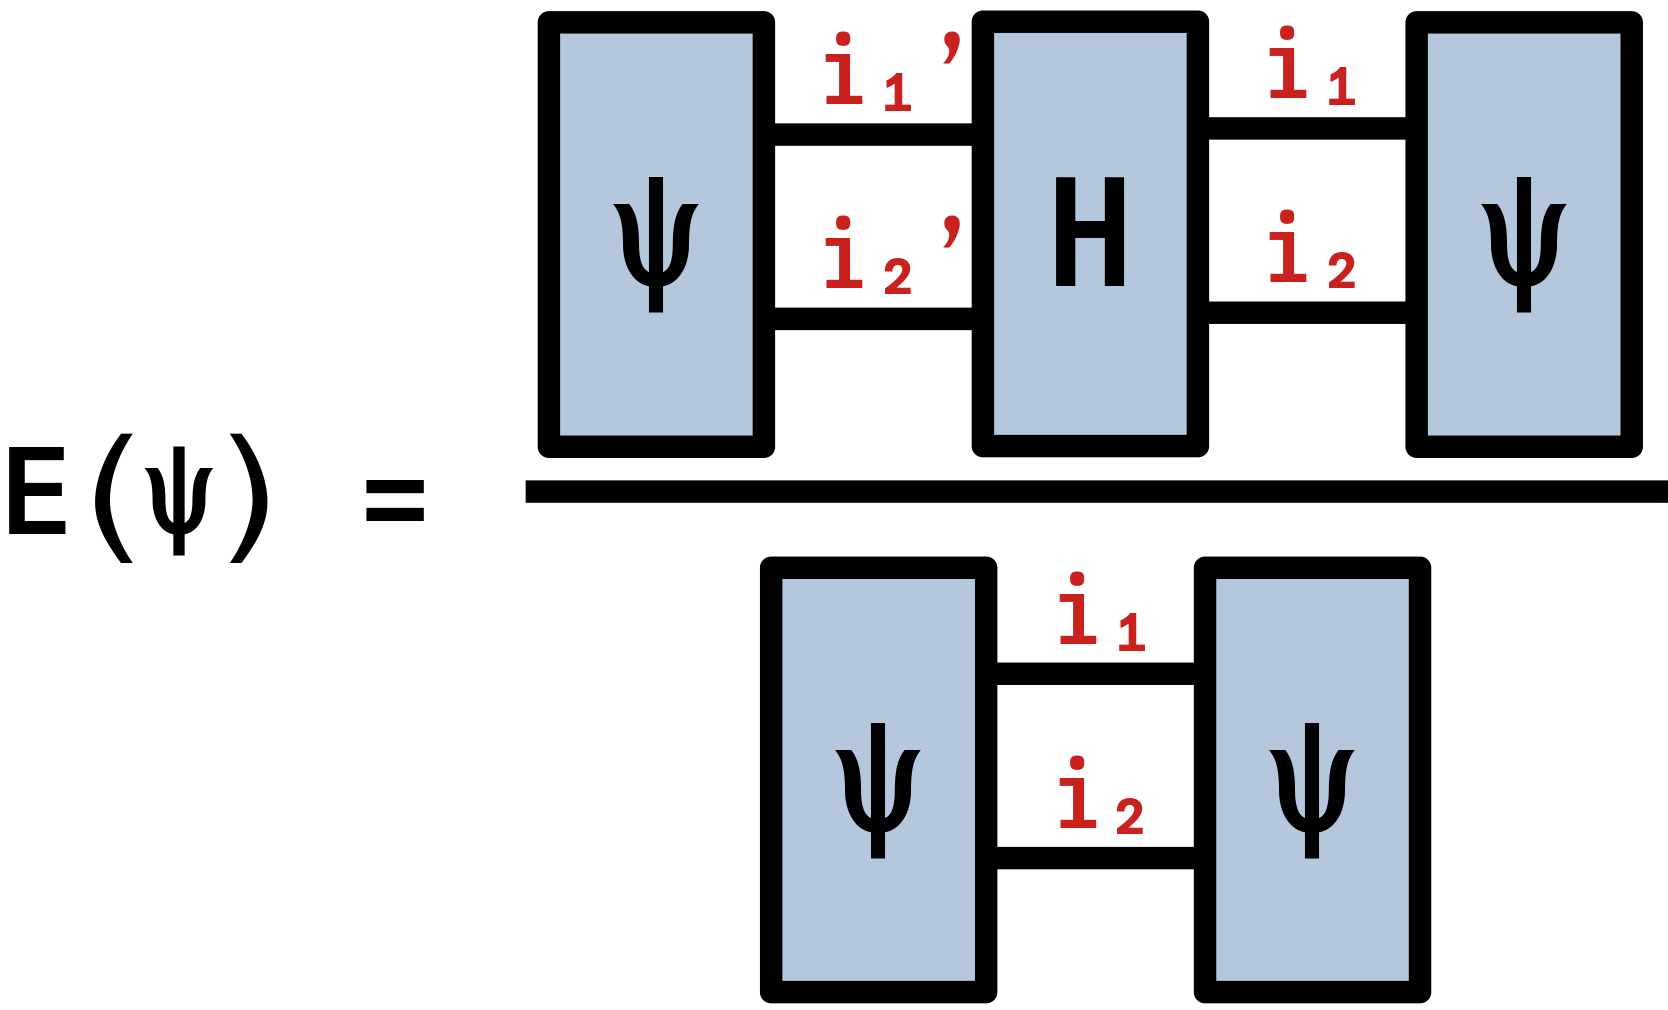
\includegraphics[width=1.0\textwidth]{
  slides/assets/psi12Hpsi12.png
}
\end{center}
\vspace*{0.0cm}
\end{onlyenv}

\begin{onlyenv}<3-3>
Simple gradient descent. \\
Must provide function f(x) \\
to minimize and $\partial$f(x), \\
the gradient of f at x. \\
~
$\gamma$ is the gradient \\
descent step size. \\
\end{onlyenv}

\begin{onlyenv}<4->
\vspace*{0.0cm}
\begin{center}
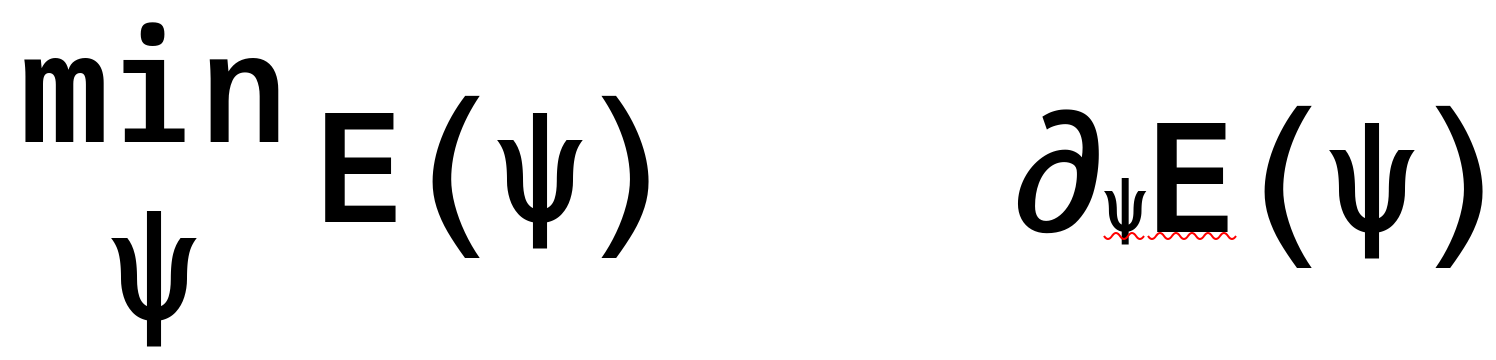
\includegraphics[width=1.0\textwidth]{
  slides/assets/min_grad_E_psi.png
}
\end{center}
\vspace*{0.0cm}
\end{onlyenv}

\end{column}

\end{columns}

\end{frame}
